\documentclass{beamer}
\usepackage[utf8]{inputenc}
\usepackage[ngerman]{babel}
\usetheme{Warsaw}  %% Themenwahl
\usepackage{graphicx}
%keine navigationsbar, da für 3 slides unnötig
\beamertemplatenavigationsymbolsempty
%für schönere Einheiten
\usepackage{siunitx}
%package für farben
\usepackage{color}

\title{Born-Oppenheimer MD}
\subtitle{Modellierung einer Diels-Alder Reaktion}
\author{N. Baumann \and L. Knirsch \and J. Sammet}
\date{29. Mai 2019}

\begin{document}

%Startfolie
\begin{frame}
  \titlepage
\end{frame}


%Folie 1
\begin{frame}
  \frametitle{Born-Oppenheimer Molecular Dynamics (BOMD)}
  \begin{itemize}
    \item Problem: Klassische Kraftfelder können keine chem. Reaktionen beschreiben $\rightarrow$ Quantenmechanik benötigt!
    \item Kräfte- und Energieberechnung mittels \textbf{semi-empirischer Methoden} anstatt des Lennard-Jones-Potentials möglich
    \item Anwendung: Modellierung einer Diels-Alder-Reaktion
    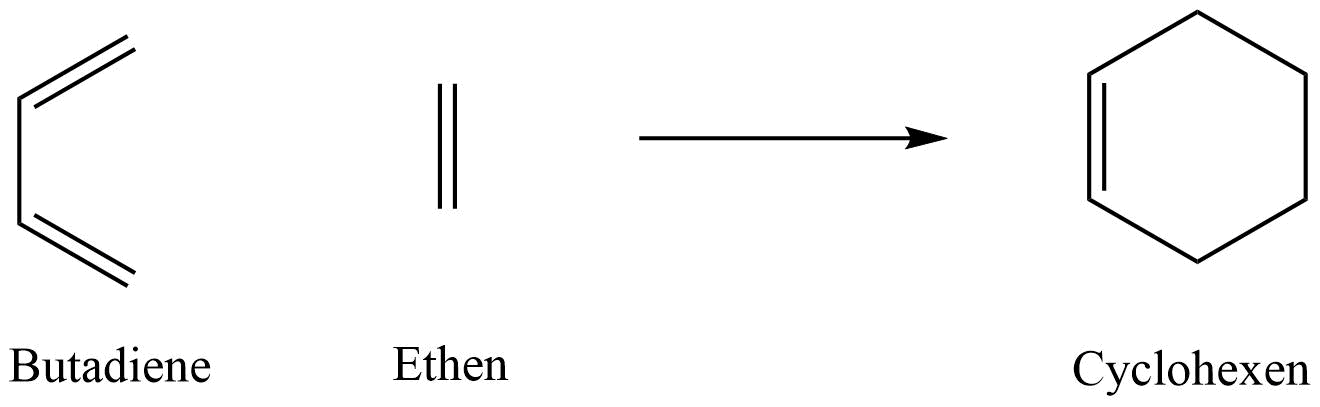
\includegraphics[scale=0.15]{DielsAlder.png}
    \item Kollision der beiden Moleküle mit verschiedenen Anfangsgeschwindigkeiten
    \item Minimale Geschwindigkeit bestimmen, bei der die Reaktionsbarriere überwunden wird $\rightarrow$ Reaktionsbarriere abschätzen
  \end{itemize}
\end{frame}


%Folie 2
\begin{frame}
  \frametitle{Implementierung}
  \begin{itemize}
    %\item Bibliothek zur Berechnung der Kräfte bereits gegeben.
    \item Essentiell: Kopplung der bereitgestellten Bibliothek an \texttt{mdatom}.
    \item Schwierigkeiten:
    \begin{itemize}
      \item Einheiten
      \item Dateiformate (\texttt{.inp \& .xyz})
      \item Anfangswerte festlegen, d.h. Positionen, Winkel und Geschwindigkeiten der Moleküle.
      \item \texttt{mdatom} akzeptiert nur Atome der gleichen Sorte, leichte Anpassungen (Massen- und Energieberechnungen) nötig.
    \end{itemize}
    \item Überprüfung: Erstellen von Animationen mittels Avogadro, einer Molekül-Viewing-Software. Alternativ: Bindungsordnung mit Bibliothek berechnen.
  \end{itemize}


\end{frame}


%Folie 3
\begin{frame}
  \frametitle{Resultate}
  \begin{itemize}
    \item Literaturwert:
    \begin{itemize}
      \item \small Experimentell: $E_A = 115.1 \si{\kilo\joule\per\mol}$
      \\  \tiny{Quelle: Discuss. \textit{Faraday Soc. \textbf{1951}, 10, 198-213}}
      \item \small genauere quantenchemische Rechnungen: $E_A = 106.3 \si{\kilo\joule\per\mol}$
      \\  \tiny{Quelle: \textit{J. Org. Chem. \textbf{1989}, 54(12), 2931-2935}}
    \end{itemize}
    \item \normalsize minimale kin. Energie für Reaktion: $E_{kin}=\frac{1}{2}v^2\sum_{i=1}^{16}m_i$
    \begin{itemize}
      \item $E_{kin}(DFTB) \approx 58.1 \si{\kilo\joule\per\mol}$
      \item $E_{kin}(PM6) \approx 101.2 \si{\kilo\joule\per\mol}$
    \end{itemize}
    \begin{figure}
      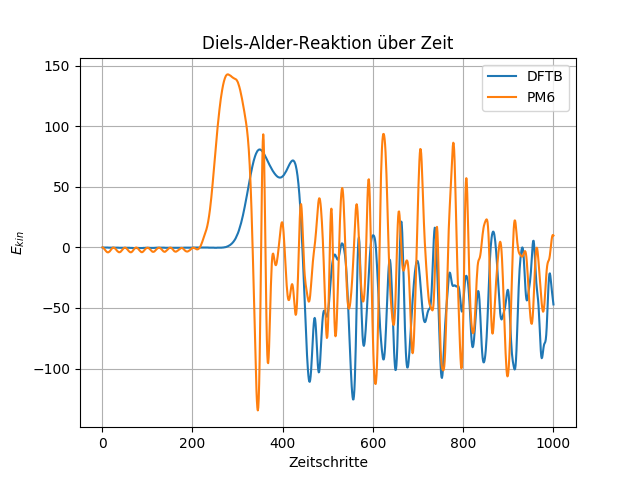
\includegraphics[scale=0.37]{dftb1_19pm61_57Data.png}
    \end{figure}
  \end{itemize}
\end{frame}



\end{document}
